\documentclass[10pt]{article}

\usepackage{tikz}
\usepackage{tkz-graph}
\usetikzlibrary{shapes,arrows}

\newcommand{\entrynode}[1]{
  \SetVertexNormal[Shape      = circle,
                   FillColor  = black,
                   LineWidth  = 0pt,
                   MinSize    = 0pt]
  \Vertex[L={\tiny\,}]{#1}
  \SetVertexNormal[Shape      = circle,
                   FillColor  = white,
                   LineWidth  = 2pt]
}

\SetUpEdge[lw         = 1.5pt,
           color      = black,
           labelcolor = white,
           labeltext  = red,
           labelstyle = {sloped,draw,text=blue}]

\tikzset{node distance = 2cm}



\begin{document}
\thispagestyle{empty}
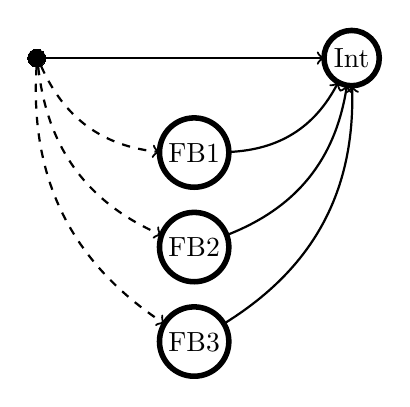
\begin{tikzpicture}
  \entrynode{A}
  \Vertex[x=4,y=0,L=Int]{B}
  \Vertex[x=2,y=-1.2,L=FB1]{C}
  \Vertex[x=2,y=-2.4,L=FB2]{D}
  \Vertex[x=2,y=-3.6,L=FB3]{E}
  \tikzstyle{EdgeStyle}=[->]
  \Edge(A)(B)
  \tikzstyle{EdgeStyle}=[dashed, bend right, ->]
  \Edge(A)(C)
  \Edge(A)(D)
  \Edge(A)(E)
  \tikzstyle{EdgeStyle}=[bend right, ->]
  \Edge(C)(B)
  \Edge(D)(B)
  \Edge(E)(B)
\end{tikzpicture}
\end{document}

